\chapter{Evaluation}

This chapter will discuss the evalution and testing of the system and its components. The next sections will cover the evaluation of the frontend, backend and the LLM used. This chapter will then conclude with a discussion on the client feedback received at the end of the project.

\section{Frontend Testing}

Frontend testing was mainly conducted through manual testing, done at the same time as the development of said components. While initially the plan was to use automated testing, the time constraints, complexity of components and lack of experience with any testing frameworks led to the decision to use manual testing instead. 

To ensure some level of robustness in the testing procedure, a checklist or a list of test cases was created for every created component. After finishing development, this list would then be used to ensure the component wasa working as intended. To have a more structured approach, the test cases were usually written using the Gherkin syntax, which follows the Given-When-Then format, allowing for better definition of the test cases \parencite{gherkin}. 

An example of some test cases for the selection of records to be shared in a share link is shown below:

\begin{lstlisting}[language=Gherkin, caption=Test cases for selecting records to be shared in a share link]
    Feature: Record selection for share link

    Scenario: User selects all record types to be shared
        Given the user is on the share link page
        When the user selects the top checkbox to select all record types
        Then all record types should be selected for sharing
        And the all children checkboxes should be selected as well 
    
    Scenario: User selects specific record types to be shared
        Given the user is on the share link page
        When the user selects a specific record type to be shared
        Then only the selected record types should be selected for sharing
        And the respective children checkboxes should all be selected as well

    Scenario: User selects specific children records to be shared
        Given the user is on the share link page
        When the user selects specific children records to be shared
        Then only the selected children records should be selected for sharing
        And the respective parent checkbox should not be selected
        And the top child checkbox should not be selected
\end{lstlisting}

And the respective frontend result of these test cases can be seen in figures~\ref{fig:test1},~\ref{fig:test2} and~\ref{fig:test3}. The first figure shows the selection of all record types, the second figure shows the selection of specific record types and the third figure shows the selection of specific children records.

\begin{figure}[htbp]
    \centering
    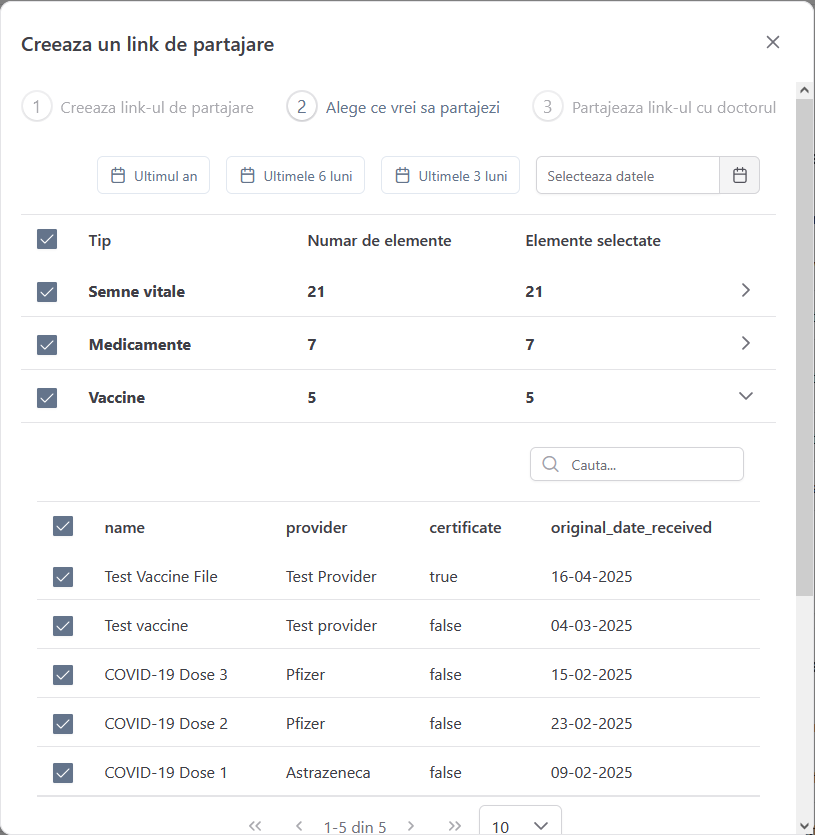
\includegraphics[width=\textwidth]{TestCase_All.png}
    \caption{Test Scenario \#1}\label{fig:test1}
\end{figure}


\begin{figure}[htbp]
    \centering
    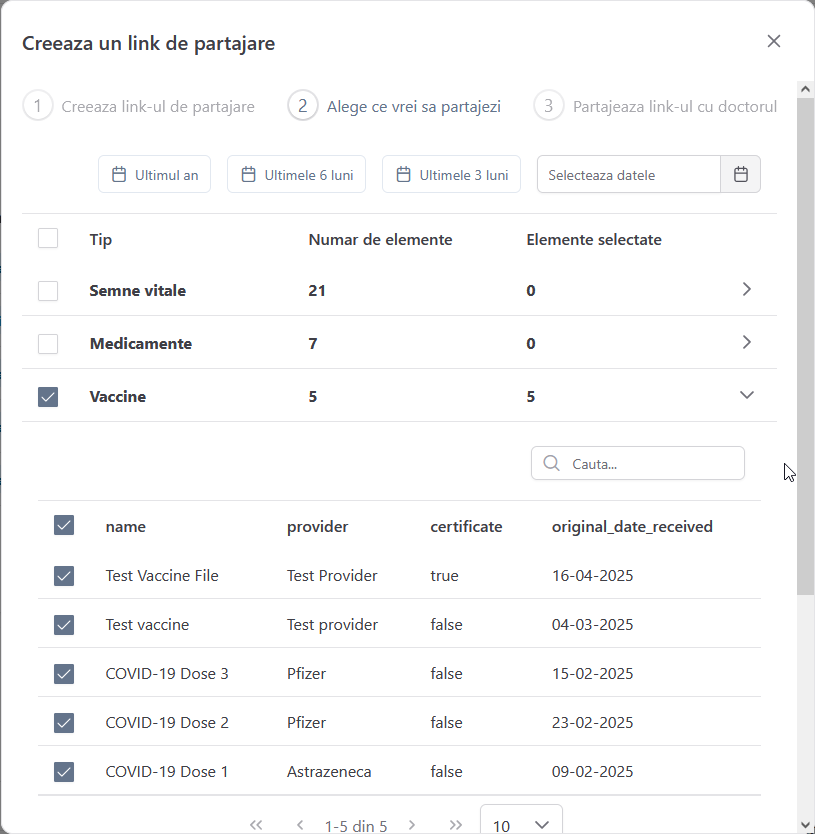
\includegraphics[width=\textwidth]{TestCase_One.png}
    \caption{Test Scenario \#2}\label{fig:test2}
\end{figure}

\begin{figure}[htbp]
    \centering
    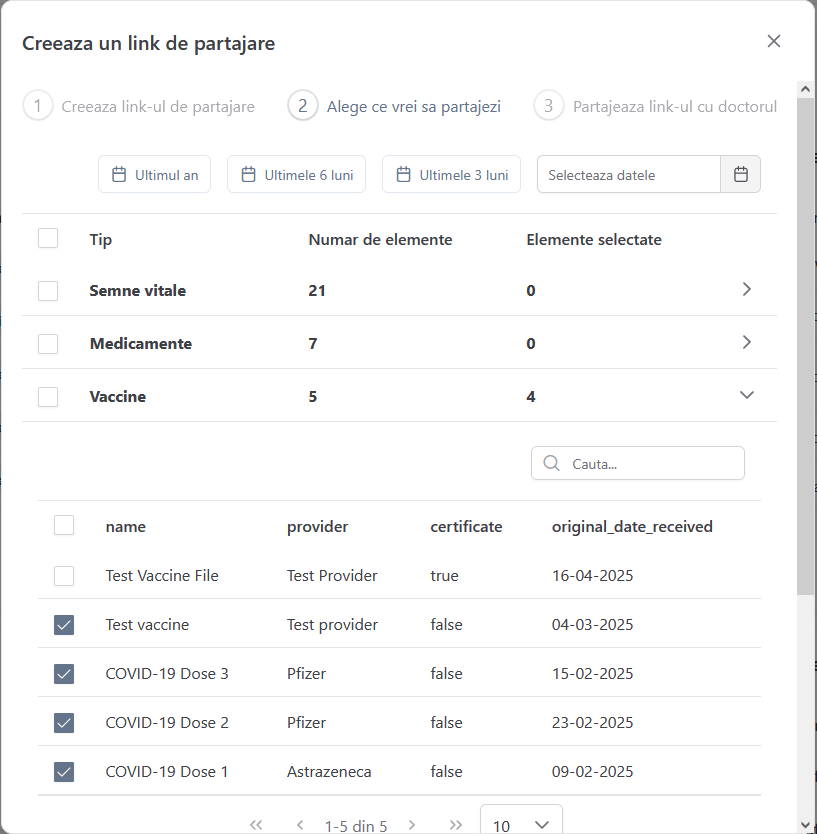
\includegraphics[width=\textwidth]{TestCase_SomeChild.png}
    \caption{Test Scenario \#3}\label{fig:test3}
\end{figure}

\FloatBarrier{}

In addition to the test cases, a site map was created to track all the pages and their respective components, with relationships showing how each page and component is related to each other. This was done to ensure that all components were created and tested properly. In the end, it allowed for a better, high-level overview of the system and its parts, but also for tracking of the overall progress of the project. The site map can be seen in figure~\ref{fig:sitemap}.

\begin{figure}[htbp]
    \centering
    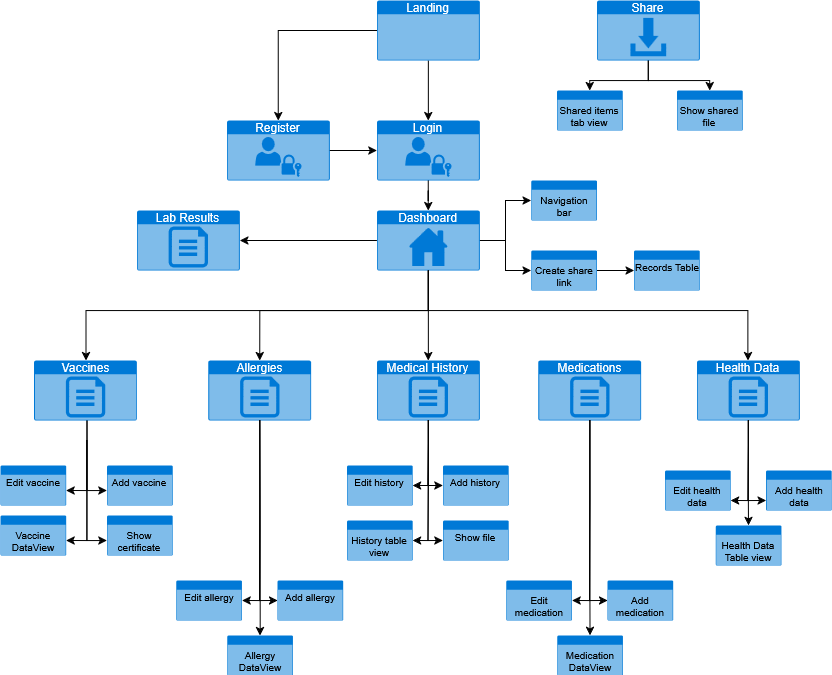
\includegraphics[width=\textwidth]{SiteMap.png}
    \caption{PHR System Site Map}\label{fig:sitemap}
\end{figure}

\FloatBarrier{}

\section{Backend Testing}

The backend testing part was also done manually. Thankfully, the backend was less complex than the frontend, so the testing was easier and faster to do. Additionally, much of backend's functionality was already tested simultaneously with the frontend testing, as it was dependent on the backend to work properly. As such, many of the test cases were already covered in the frontend testing.

However, to ensure that the backend was working as intended, additional tests were done using Postman while the API was being developed. This allowed for testing of the endpoints without relying on the frontend components being created. The tests were done by sending requests to the API and checking the responses, and comparing them with the expected results. 

An example of how an endpoint was tested will be shown now. An example endpoint can be seen below:

\begin{lstlisting}[language=Python, caption=Example endpoint for checking a share link for expiration time]
    @router.get("/share/{share_code}", status_code=status.HTTP_200_OK)
@limiter.limit("5/minute")
async def check_share_token(
    request: Request,
    share_code: str,
    session: Session = Depends(get_session)
):
    share_token = session.exec(select(ShareToken).where(ShareToken.share_code == share_code)).first()
    
    if not share_token:
        raise HTTPException(status_code=status.HTTP_404_NOT_FOUND, detail="Share token not found")
    
    if share_token.expiration_time < datetime.now():
        raise HTTPException(status_code=status.HTTP_410_GONE, detail="Share token has expired")
    
    return {
        "valid": True
    }
\end{lstlisting}

This endpoint checks if a share link is valid and if it has expired. The endpoint takes in a share code and checks if it exists in the database. If it does, it checks if the expiration time is still valid. If both checks pass, it returns a valid response. If either check fails, it raises an HTTP exception with the appropriate status code and message.

As such, for this endpoint, 3 test cases can be created: one where the share code is not valid, another where the code is valid but the expiration time is not valid and a third one where everything is valid. The test cases in Postman can be seen in figures~\ref{fig:postman1},~\ref{fig:postman2} and~\ref{fig:postman3}.

\begin{figure}[htbp]
    \centering
    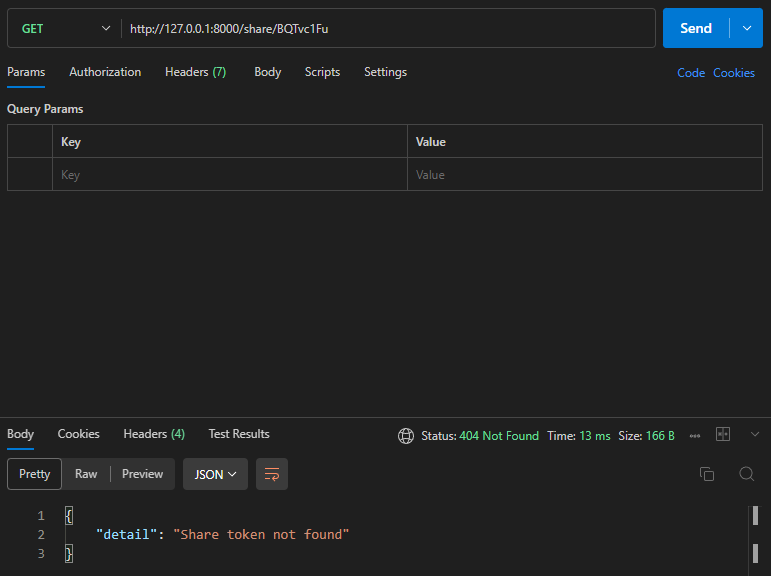
\includegraphics[width=\textwidth]{PostmanNotFound.png}
    \caption{Postman test --- share token not found}\label{fig:postman1}
\end{figure}

\begin{figure}[htbp]
    \centering
    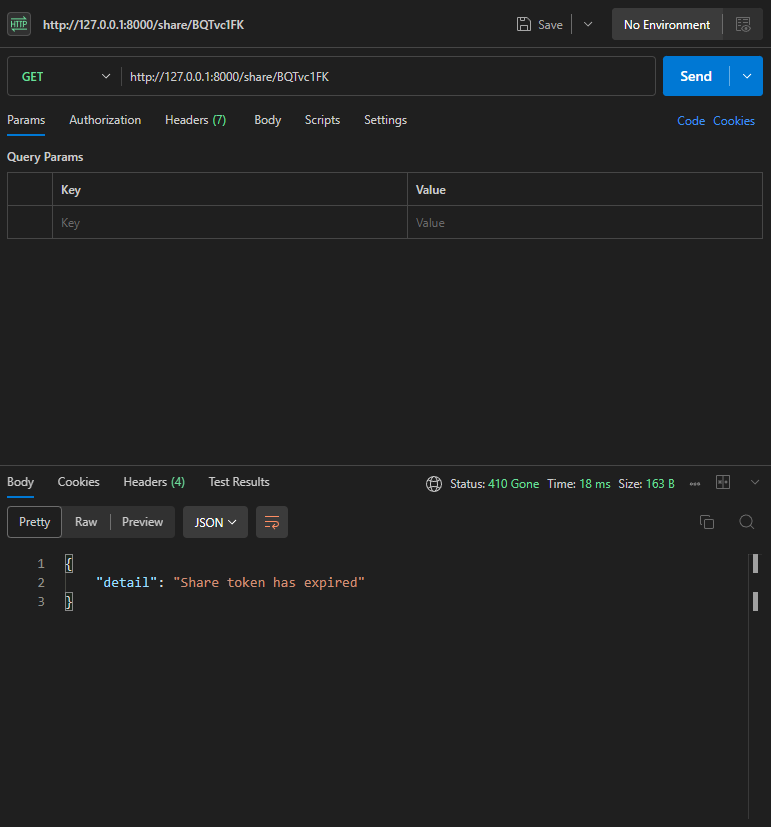
\includegraphics[width=\textwidth]{PostmanExpired.png}
    \caption{Postman test --- share token expired}\label{fig:postman2}
\end{figure}

\begin{figure}[htbp]
    \centering
    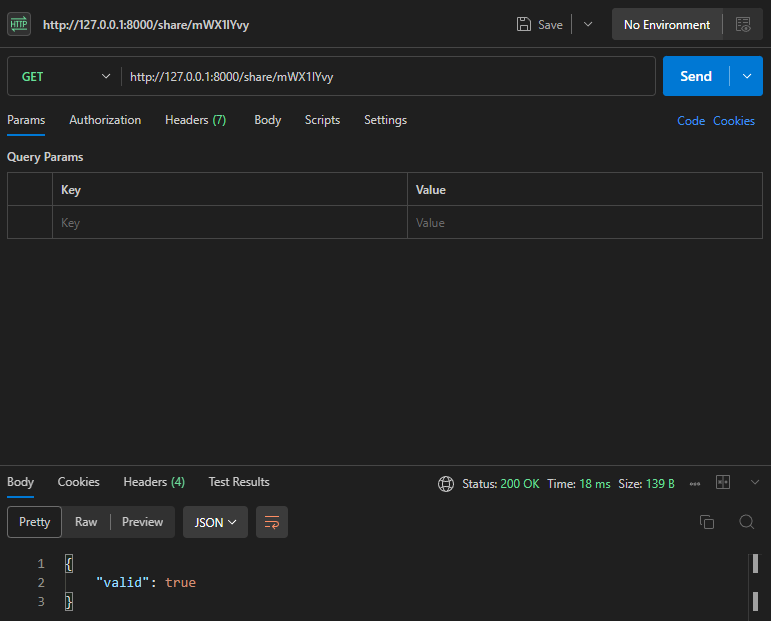
\includegraphics[width=\textwidth]{PostmanOK.png}
    \caption{Postman test --- share token valid}\label{fig:postman3}
\end{figure}

\FloatBarrier{}

\section{LLM Evaluation}

As previously mentioned in the Development chapter, the MLLM used in this project was Gemini 2.0 Flash. One of the main reasons for using this LLM was its generous free tier, which allowed for up to 15 requests per minute with a maximum of 1,000,000 tokens per minute. Alongside the generous free tier, the model also sported robust multimodal capabilities, which was crucial for processing lab results, which were often in PDF or image format. 

However, it is also important to note that while the free tier and its multimodal capabilities were a big factor in choosing this model, it was also chosen for its performance and speed, which rivaled that of other, similarly sized models. As of writing this section, Gemini 2.0 Flash occupies a spot in the top 10 of the Chatbot Arena leaderboard for both language and vision tasks, authored by \textcite{chatbotarena}. As described by its authors, the leaderboard is an `open platform for crowdsourced AI benchmarking', which generates live leaderboards based on user feedback from comparing responses from different models. As such, it is quite likely that this leaderboard is a good indicator of the performance of the models, and good place to compare them.

To ensure the MLLM was working as intended and was up to the task, the same prompt used in the actual system was used to test the model across multiple lab result documents from various institutions. Documents from different institutions such as labs and hospitals were used to ensure that the model was able to handle different formats of the document and the language used within it. 

Three different documents were used for evaluation --- 2 from labs and 1 from a private hospital. The labs and the hospital were chosen for their popularity and a wide network of testing sites across the whole country \parencite{alfalab, synevo, medpark}. The anonymised documents, alongside their extracted results, can be seen in the following figures:~\ref{fig:synevo},~\ref{fig:alfalab} and~\ref{fig:medpark}.

\begin{figure}[ht]
    \centering
    \subfloat[Lab document]{%
        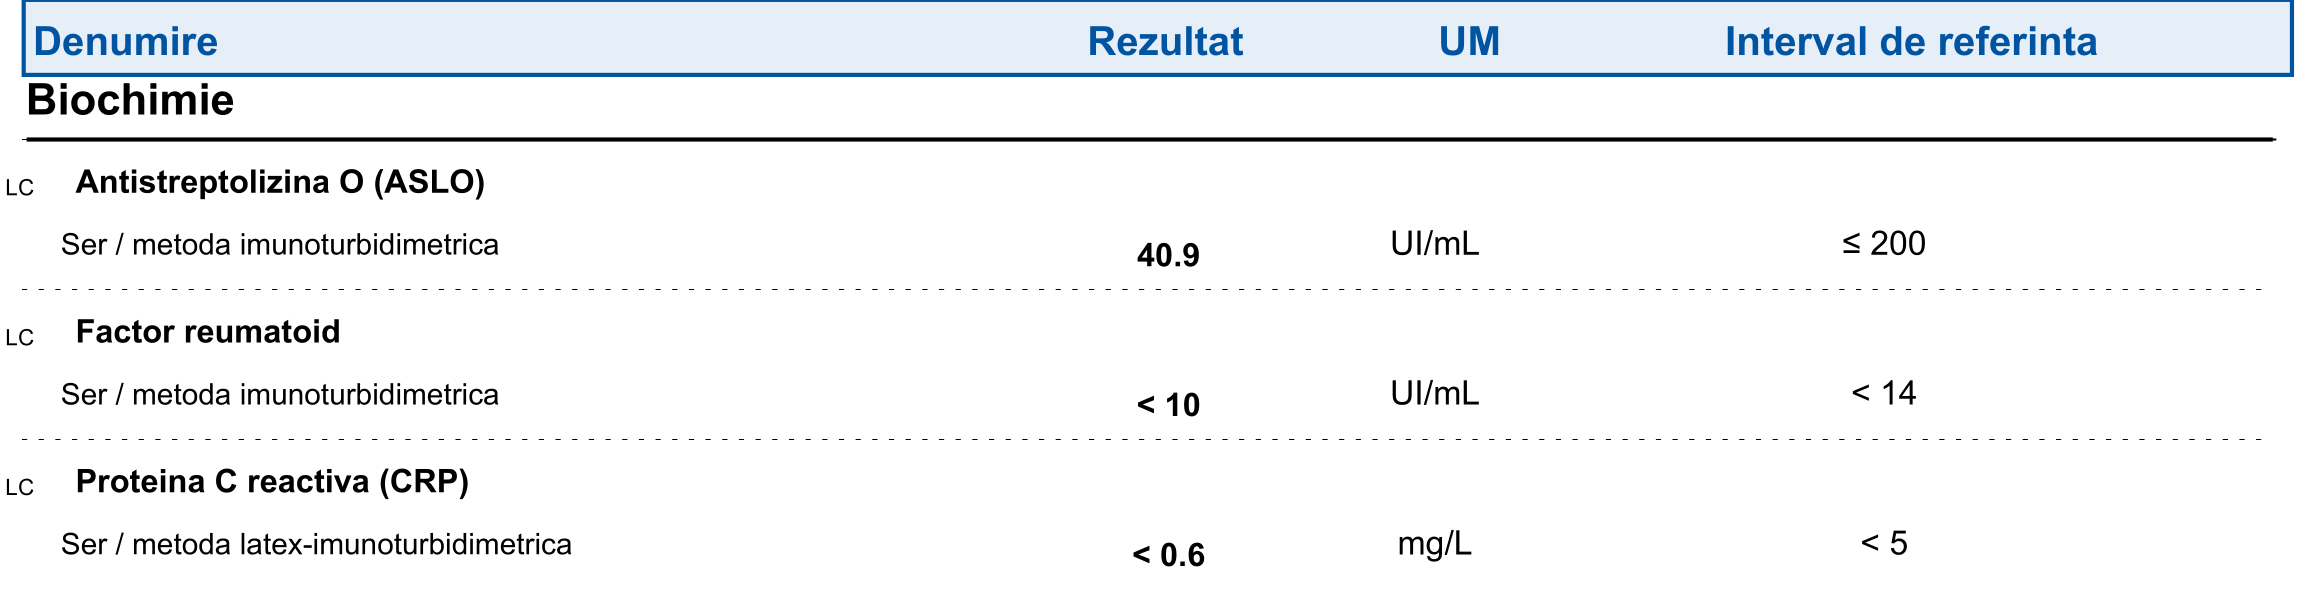
\includegraphics[width=0.9\textwidth]{Synevo_edited.png}%
    }
    \\[\baselineskip]
    \subfloat[Extraction result]{%
        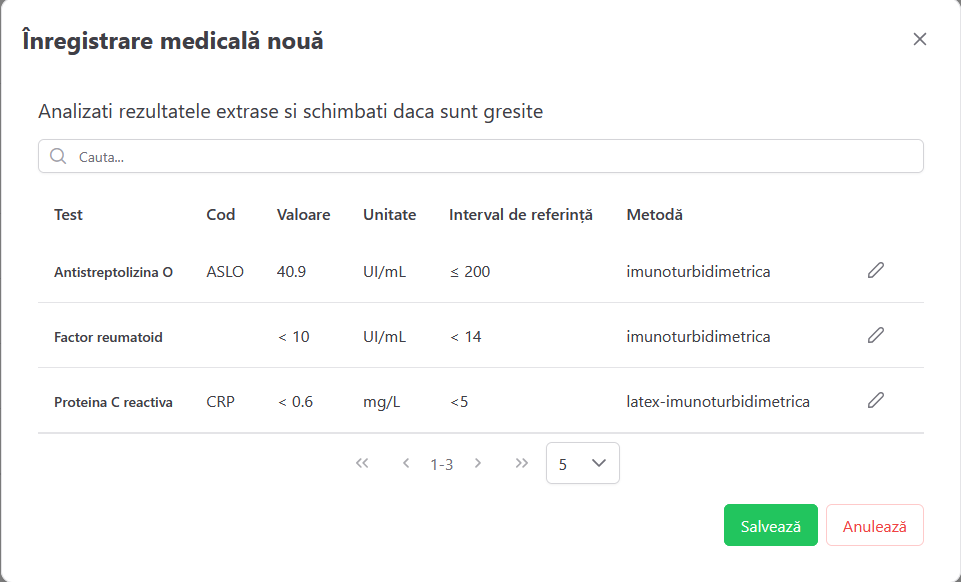
\includegraphics[width=0.9\textwidth]{Synevo_result.png}%
    }
    \caption{Synevo extraction results}\label{fig:synevo}
\end{figure}

\begin{figure}[ht]
    \centering
    \subfloat[Lab document]{%
        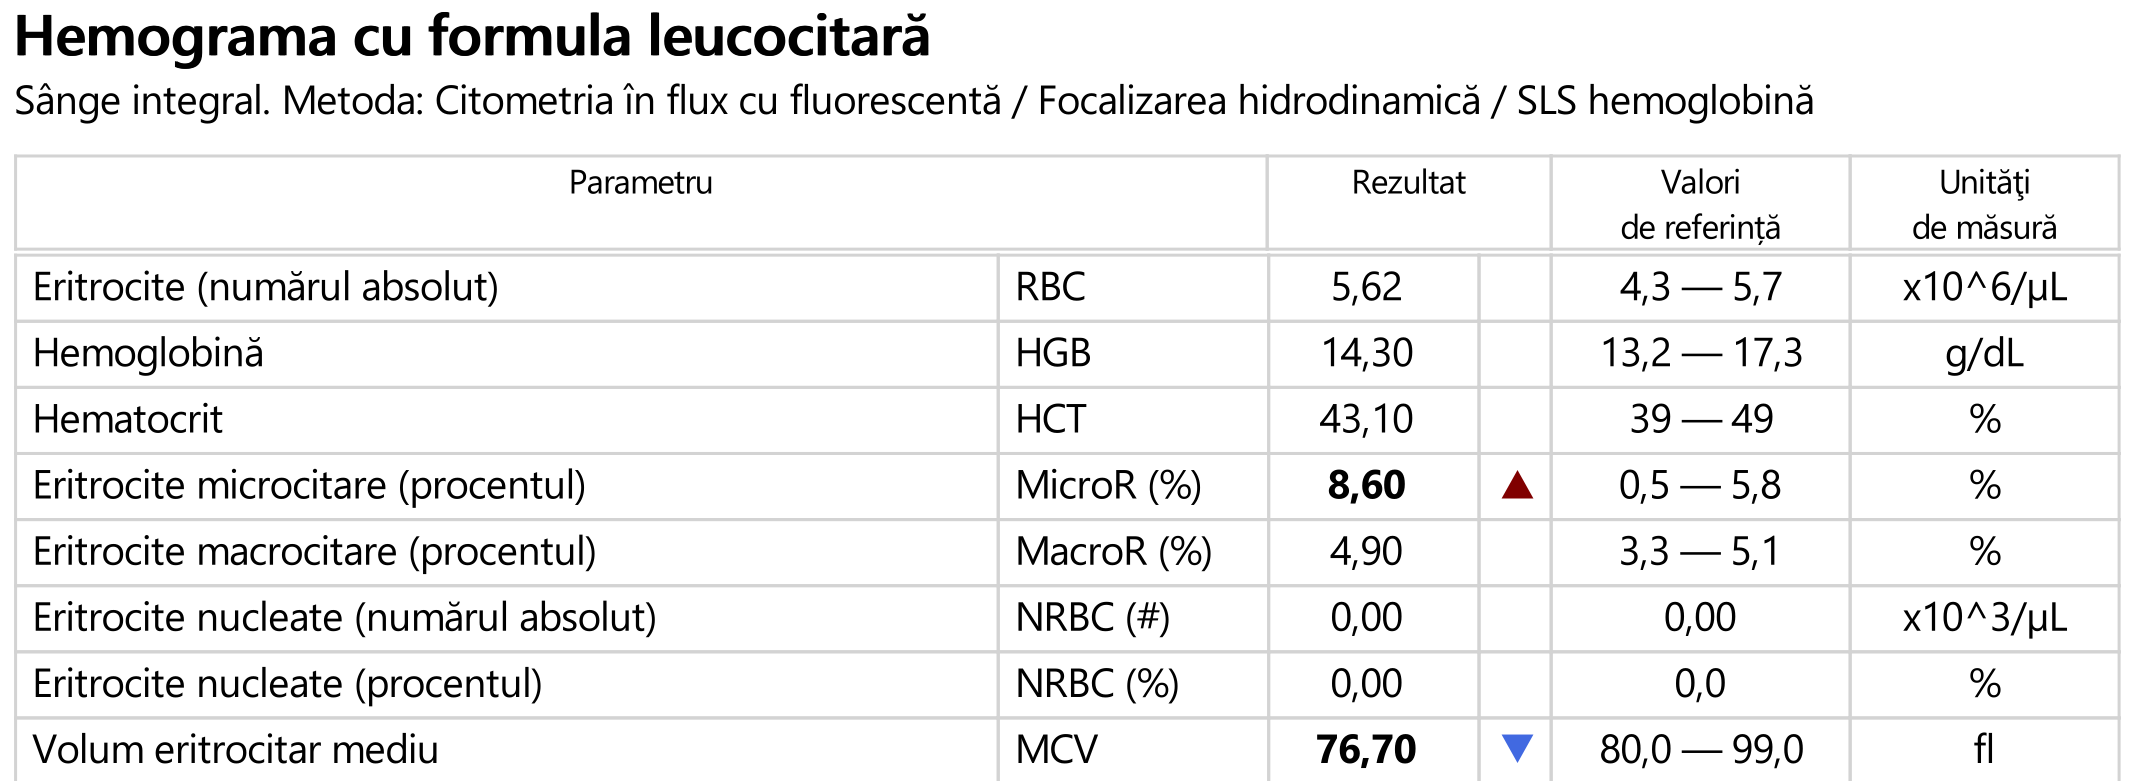
\includegraphics[width=0.9\textwidth]{Alfalab_edited.png}%
    }
    \\[\baselineskip]
    \subfloat[Extraction result]{%
        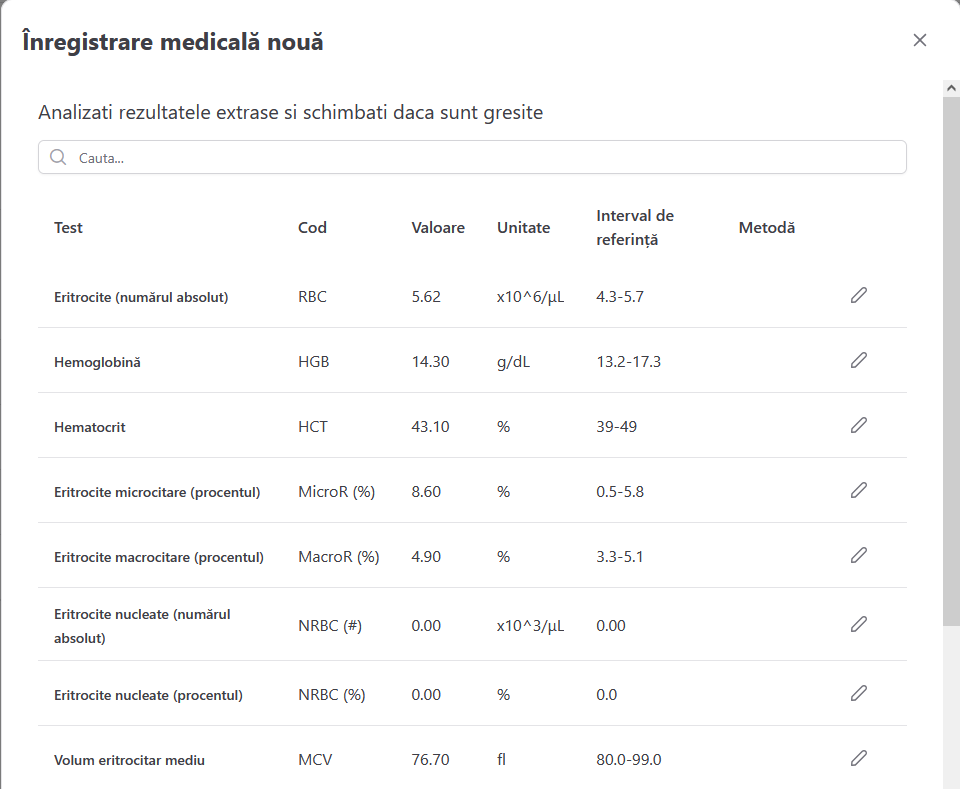
\includegraphics[width=0.9\textwidth]{Alfalab_result.png}%
    }
    \caption{Alfalab extraction results}\label{fig:alfalab}
\end{figure}

\begin{figure}[ht]
    \centering
    \subfloat[Lab document]{%
        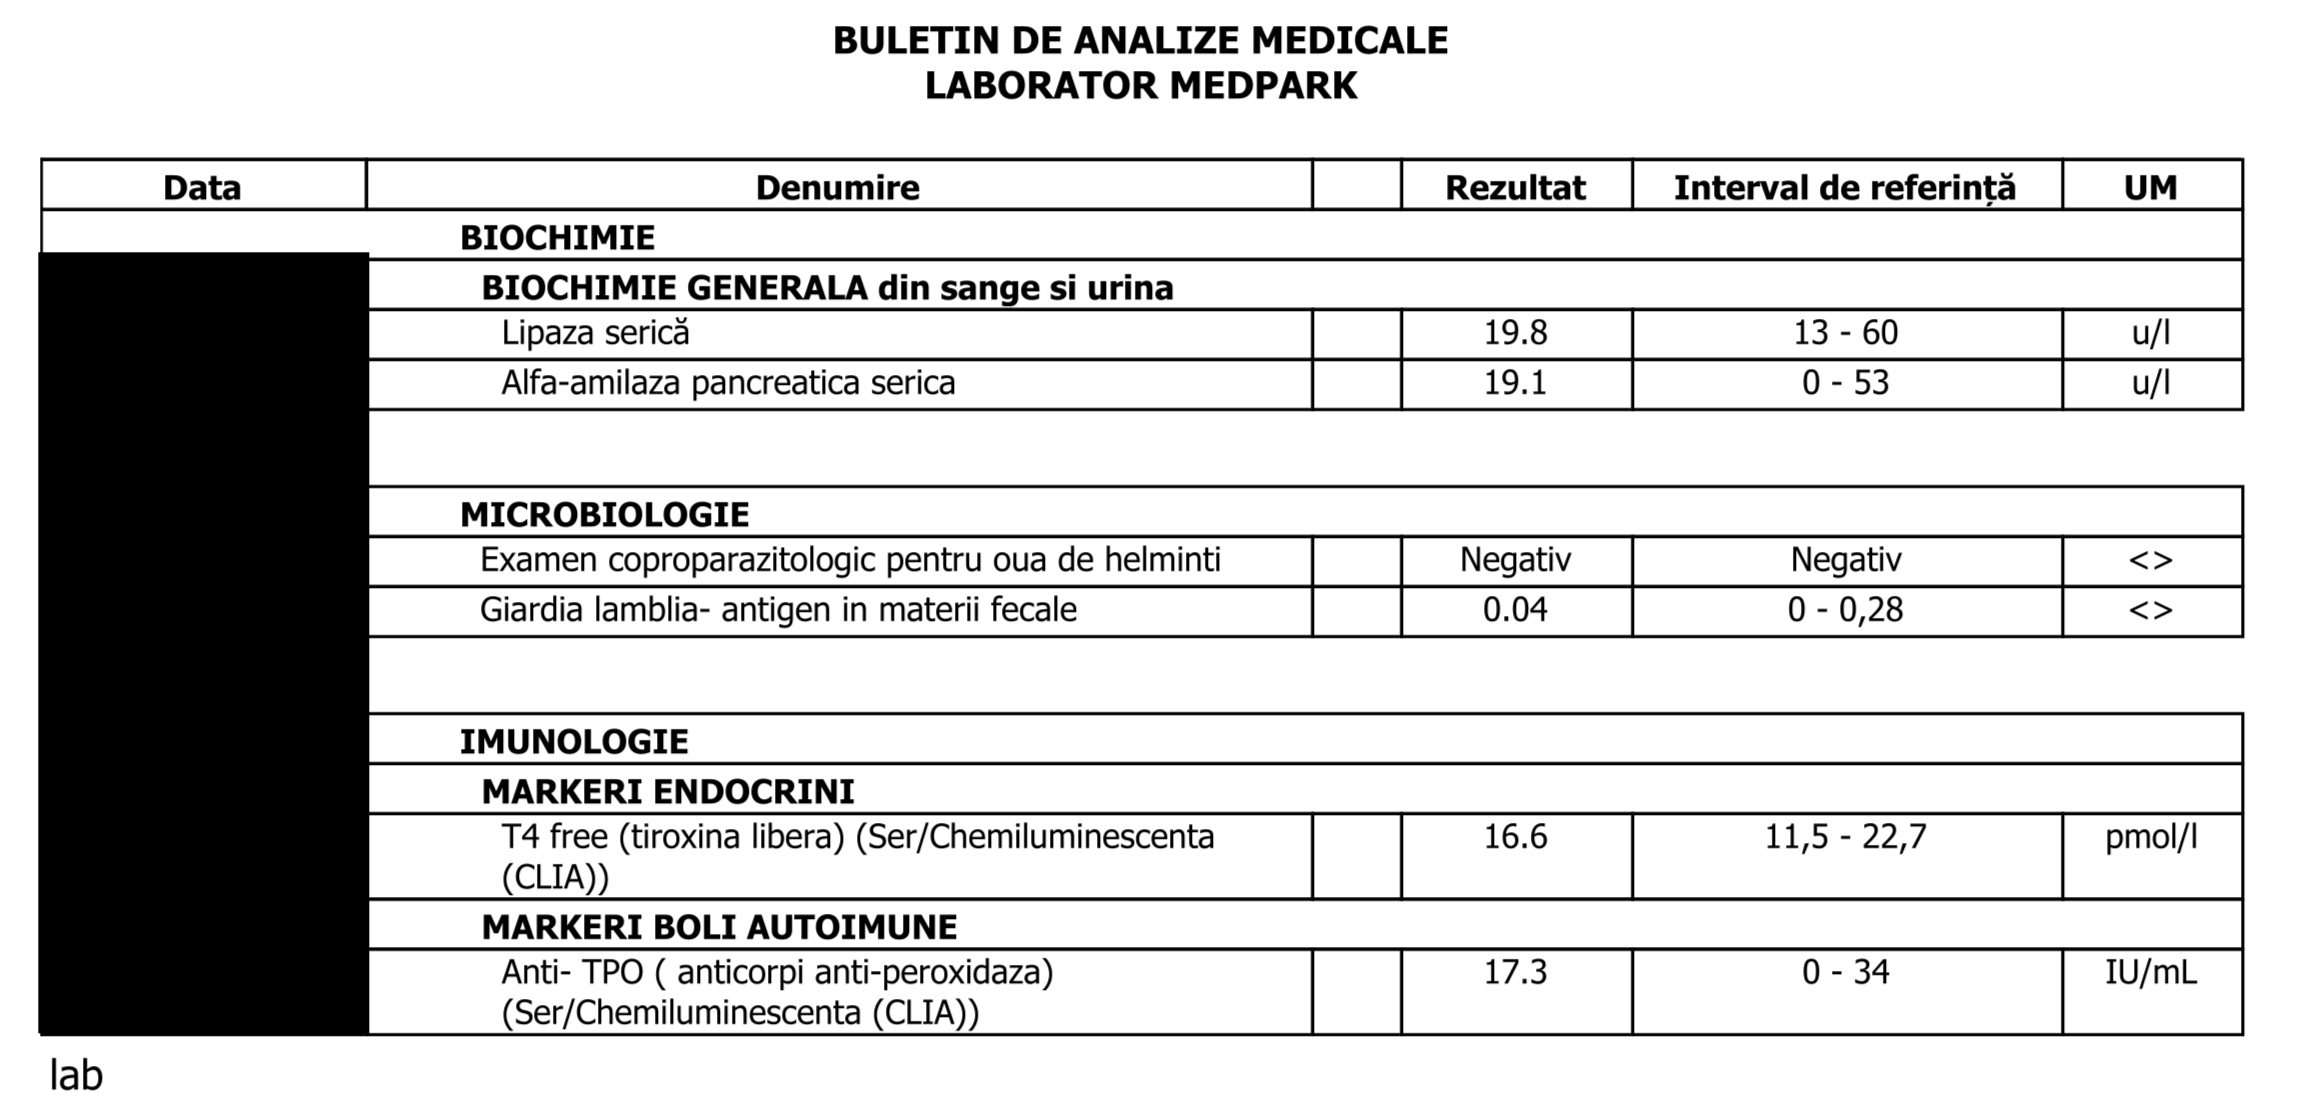
\includegraphics[width=0.9\textwidth]{Medpark_edited.png}%
    }
    \\[\baselineskip]
    \subfloat[Extraction result]{%
        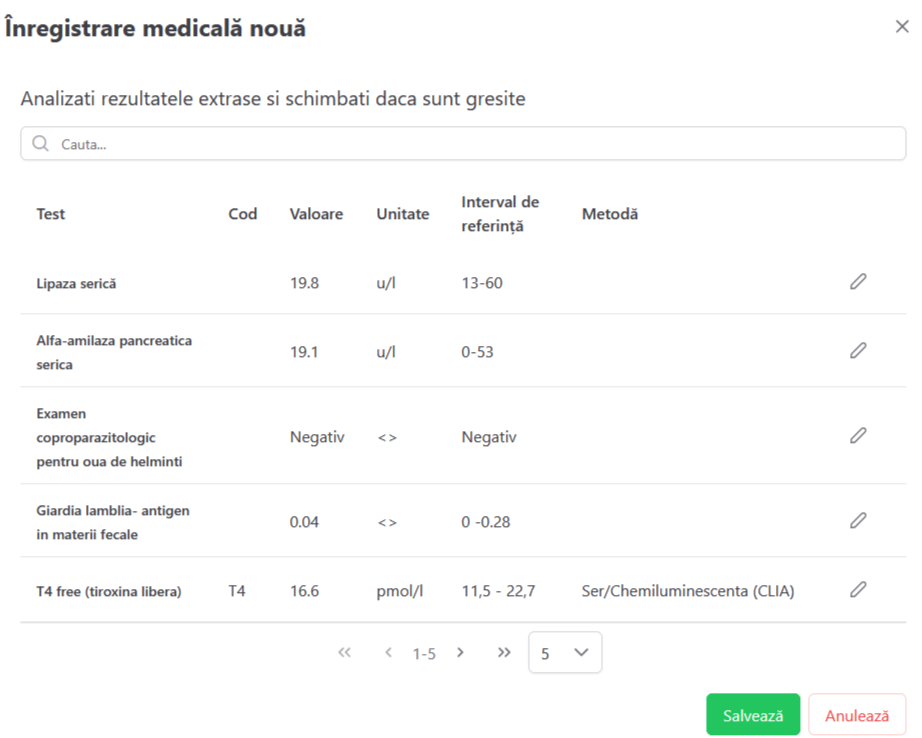
\includegraphics[width=0.9\textwidth]{Medpark_result.png}%
    }
    \caption{Medpark extraction results}\label{fig:medpark}
\end{figure}

\FloatBarrier{}

As it can be seen by the results, the model was able to extract the lab results and their details such as code, reference range, unit and even method. These excellent results were achieved with a single, common prompt and delivered consistent results across all 3 documents, whether they were edited in any way or not. In conclusion, the model seemed to be an excellent choice for the task at hand, and these results confirmed that Gemini 2.0 Flash was indeed a suitable choice for extracting lab results from documents.

\section{Stakeholders feedback}

To round up this section and the development of the system, feedback was collected from involved stakeholders regarding its performance and usability. The feedback was collected through virtual meetings, where the system was presented in a live demo format. After the presentation, stakeholders were allowed to ask any further questions and at the end they were  provided feedback on the developed system and its future potential in the digital healthcare industry in Moldova.

There was no formal feedback collection process, nor a structured questionnaire, with stakeholders being encouraged to express their opinions in a free format. Some feedback excerpts can be seen below, with the names of the stakeholders anonymised. The full feedback can be found in the appendix~\ref{sec:full_feedback}.


Feedback 1, from a medical doctor specialised in digital healthcare applications:

\begin{quotation}
    `I appreciated the concept of the project and the way all essential components of a Personal Health Record were integrated: general, clinical, and paraclinical data, consultations, physician access, and data security. The platform is strongly patient-centered, enhancing access to personal medical data and significantly contributing to patient empowerment\dots From my perspective as a medical doctor specialized in public health and an expert in digital transformation of healthcare, I see great potential in this project and I am committed to offering the necessary support for its further development'
\end{quotation}

Feedback 2, from a patient and healthcare user:

\begin{quotation}
    `I was really impressioned with the application on the digital health records book you have developed and presented to me. As a BA you have managed to capture the most important needs and then translated them into useful features included in the solution developed\dots By developing this solution you have given a new opportunity to Moldova to make one big step forward to the digitisation, and hope it will be largely used by moldovans as the country offers them also other related nice opportunities like high speed internet access and good coverage by 5G network'
\end{quotation}